\documentclass[sigconf,9pt]{acmart}

\usepackage{booktabs} % For formal tables
\usepackage{listings}
\lstset{
  basicstyle=\scriptsize,
}
\usepackage{tikz}
\usetikzlibrary{arrows,positioning,fit,calc,decorations.markings}
\usepackage{pgfplots}
\pgfplotsset{compat=newest} % Allows to place the legend below plot
\usepgfplotslibrary{units} % Allows to enter the units nicely
\usepackage{url}
\usepackage{multirow}
\usepackage{graphicx}

\newcommand{\elq}{ELQ}
\newcommand{\code}[1]{\texttt{#1}}


% Copyright
%\setcopyright{none}
%\setcopyright{acmcopyright}
%\setcopyright{acmlicensed}
\setcopyright{rightsretained}
%\setcopyright{usgov}
%\setcopyright{usgovmixed}
%\setcopyright{cagov}
%\setcopyright{cagovmixed}


% DOI
% \acmDOI{10.475/123_4}

% ISBN
% \acmISBN{123-4567-24-567/08/06}

%Conference
% \acmConference[WOODSTOCK'97]{ACM Woodstock conference}{July 1997}{El
%   Paso, Texas USA}
% \acmYear{1997}
% \copyrightyear{2016}
%
% \acmPrice{15.00}


\begin{document}
\title{Modular Responsive Web Design Using\\ Element Queries: An Experience Report}

\author{Lucas Wiener}
\affiliation{%
  \institution{EVRY AB, Sweden}
  \streetaddress{Ekensbergsvägen 113}
  \city{Solna}
  \postcode{171 79}
}
\email{lucas.wiener@evry.com}

\author{Tomas Ekholm}
\affiliation{%
  \institution{KTH Royal Institute of Technology}
  \streetaddress{Brinellvägen 8}
  \city{Stockholm}
  \postcode{114 28}
}
\email{tomase@kth.se}

\author{Philipp Haller}
\affiliation{%
    \institution{KTH Royal Institute of Technology}
    \streetaddress{Brinellvägen 8}
    \city{Stockholm}
    \postcode{114 28}
}
\email{phaller@kth.se}

% The default list of authors is too long for headers}
\renewcommand{\shortauthors}{L. Wiener et al.}

\begin{abstract}
    Responsive Web Design (RWD) enables web applications to adapt to the characteristics of different devices such as screen size which is important for mobile browsing.
    Today, the only W3C standard to support this adaptability is CSS media queries.
    However, using media queries it is impossible to create applications in a modular way, because responsive elements then always depend on the global context.
    Hence, responsive elements can only be reused if the global context is exactly the same.
    This makes it extremely challenging to develop large responsive applications, because the lack of true modularity makes certain requirement changes either impossible or expensive to realize.

    In this paper we extend RWD to also include responsive modules, i.e., modules that adapt their design based on their local context, independently of the global context.
    We present the \elq{} project which implements our approach.
    \elq{} is a novel implementation of so-called \emph{element queries} which generalize CSS media queries.
    Importantly, our design conforms to existing web specifications, enabling adoption on a large scale.
    \elq{} is designed to be heavily extensible using plugins.
    Experimental results show speed-ups of the core algorithms of up to 37x compared to previous approaches.
\end{abstract}

%
% The code below should be generated by the tool at
% http://dl.acm.org/ccs.cfm
% Please copy and paste the code instead of the example below.
%

\begin{CCSXML}
<ccs2012>
 <concept>
  <concept_id>10010520.10010553.10010562</concept_id>
  <concept_desc>Computer systems organization~Embedded systems</concept_desc>
  <concept_significance>500</concept_significance>
 </concept>
 <concept>
  <concept_id>10010520.10010575.10010755</concept_id>
  <concept_desc>Computer systems organization~Redundancy</concept_desc>
  <concept_significance>300</concept_significance>
 </concept>
 <concept>
  <concept_id>10010520.10010553.10010554</concept_id>
  <concept_desc>Computer systems organization~Robotics</concept_desc>
  <concept_significance>100</concept_significance>
 </concept>
 <concept>
  <concept_id>10003033.10003083.10003095</concept_id>
  <concept_desc>Networks~Network reliability</concept_desc>
  <concept_significance>100</concept_significance>
 </concept>
</ccs2012>
\end{CCSXML}

\ccsdesc[500]{Computer systems organization~Embedded systems}
\ccsdesc[300]{Computer systems organization~Redundancy}
\ccsdesc{Computer systems organization~Robotics}
\ccsdesc[100]{Networks~Network reliability}

% We no longer use \terms command
%\terms{Theory}

\keywords{Responsive web design, Element queries, CSS, Modularity}


\maketitle

\section{Introduction}
  Responsive Web Design (RWD) is an approach to make an application respond to the viewport size and device characteristics.
  This is currently achieved by using CSS media queries that are designed to conditionally design content by the media, such as using serif fonts when printed and sans-serif when viewed on a screen \cite{w3c_css_mq}.
  In order to reduce complexity and enable reusability, applications are typically composed of modules, i.e., interchangeable and independent parts that have a single and well-defined responsibility \cite{parnas1972criteria}.
  In order for a module to be reusable it must not assume in which context it is being used.

  In this paper we focus on the presentation layer of web applications.
  As it stands, using CSS media queries to make the presentation layer responsive precludes modularity.
  The problem is that there is no way to make a module responsive without making it context-aware, due to the fact that media queries can only target the viewport; this means that responsive modules can only respond to changes of the (global) viewport.
  Thus, a responsive module using media queries is layout dependent and has both reduced functionality and limited reusability~\cite{elq-thesis}.
  As a result, media queries can only be used for RWD of non-modular static applications.
  In a world where no better solution than media queries exists for RWD, changing the layout of a responsive application becomes a cumbersome task since it may require many responsive modules to be updated.
  The limitations of CSS with regard to compositionality are well known (as shown in the tweet below). While we do not claim to solve the whole problem, we address compositionality issues in the context of RWD.

  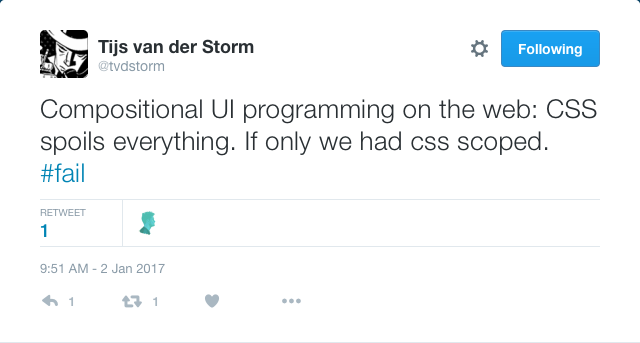
\includegraphics[scale=.35]{tweet_tvdstorm}

  \paragraph{The Problem Exemplified.}
    Imagine an application that displays the current weather of various cities as widgets, by using a weather widget module.
    The module should be responsive so that more information, such as a temperature graph over time, is displayed when the widget is big.
    When the widget is small it should only display the current temperature.
    Users should also be able to add, remove and resize widgets.

    Such an application cannot be built using media queries, since the widgets can have varying sizes independent of the viewport (e.g., the width of one widget is 30\% while another is 40\%).
    To overcome this problem we must change the application, so that widgets always have the same sizes.
    This implies that the size of the module and the media query breakpoints are coupled/intertwined, i.e. they are proportional to each other.
    The problem now is that we have removed the reusability of the weather module, since it requires the specific width that is correctly proportional to the media query breakpoints.

    Imagine a company working on a big application that uses media queries for responsiveness (i.e., each responsive module assumes to have a specific percentage of the viewport size).
    The ability to change is desired by both developers and stakeholders, but is limited by this responsive approach.
    The requirement of changing a menu from being a horizontal menu at the top to being a vertical menu on the side implies that all responsive modules break, since the assumed proportionality of each module is changed.
    Even worse, if the menu is also supposed to hide on user input, the responsiveness of the module breaks, since the layout changes dynamically.
    The latter requirement is impossible to satisfy in a modular way without element queries.

    Additionally, it is popular to define breakpoints relative to the font size so that conditional designs respect the size of the content~\cite{mq-em}.
    Media queries can only target the font size of the document root, limiting their functionality drastically.
    With element queries breakpoints may be defined relative to the font size of the targeted element.

    As we can see, even with the exemplified limited requirements there are still significant restrictions when using media queries for responsive modules.


  \paragraph{Requirements.}\label{sec:reqs}
    The desired behavior of a responsive module is having its inner design respond to the size of its \emph{container} instead of the viewport.
    Only then is a responsive module independent of its layout context.
    Realizing responsive modules requires CSS rules that are conditional upon \emph{elements}, instead of the global viewport.
    We have identified the following requirements of a solution:

    \begin{itemize}
      \item
        It must provide the possibility for an element to automatically respond to changes of its parent's properties.
      \item
        It must conform to the syntax of HTML, CSS, and JavaScript to retain the compatibility of tools, libraries and existing projects.
      \item
        It must have adequate performance for large applications that make heavy use of responsive modules.
      \item
        It must enable developers to write encapsulated style rules, so that responsive modules may be arbitrarily composed without any conflicting style rules.
    \end{itemize}
  \paragraph{Approach.}
    In this paper we extend the concept of RWD to also include responsive modules.
    The W3C has discussed such a feature under the name of \emph{element queries} given its analogy to media queries~\cite{w3c_eq_mail}.
    This paper presents a novel implementation of element queries in JavaScript named \elq{} that enables new possibilities of RWD.
    Our approach satisfies all requirements given above.
    We have released ELQ as an open-source library under the MIT license.\footnote{\url{https://github.com/elqteam/elq}}
    The implementation supports all major browsers, including Internet Explorer version 8, Chrome version 42 (the last version compatible with Android version 4), Safari version 5, and Opera version 12.

    One could argue that a solution does not need to be executed on the client side, but instead generate media queries on the server side for all modules with respect to the current application layout.
    However, this approach is insufficient, since it limits modules to applications with static layouts~\cite{elq-thesis}. Also, the generated media queries would not be able to respond to the user changing properties of elements such as layout and font size.

  \paragraph{Contributions.}
    This paper makes the following contributions:
    \begin{itemize}
      \item A new design for element queries that enables responsive modules while conforming to the syntax of HTML, CSS, and JavaScript.
      \item
        Our approach is the first to enable nested elements that are responsive in a modular way, i.e., modules fully encapsulate any styling required for RWD.
        As a side effect, responsive modules may also be arbitrarily styled with CSS independent of their context.
      \item
        An extensible architecture that enables plugins to significantly extend the behavior of ELQ, our library implementation.
        This makes it possible to create plugins in order to enable new features and to ease integration of \elq{} into existing projects.
      \item
        A new implementation that offers substantially higher performance than previous approaches.
        The implementation batch-processes DOM operations in order to avoid layout thrashing (i.e., forcing the layout engine to perform multiple independent layouts). We also provide an integration component\footnote{\url{https://github.com/elqteam/react-responsive-block}} for the React user interface library.
      \item
        A run-time cycle detection system that detects and breaks cycles stemming from cyclic rules due to unrestricted usage of element queries~\cite{elq-thesis}.
    \end{itemize}

  The rest of the paper is organized as follows.
  Section~\ref{sec:elq} introduces \elq{} and its API from a user's perspective.
  Section~\ref{sec:imp} provides an overview of the implementation of \elq{}'s element resize detection system.
  Section~\ref{sec:eval} evaluates the performance of \elq{}.
  Section~\ref{sec:case-studies} reports on case studies of using \elq{}.
  Section~\ref{sec:related} relates \elq{} to prior work.
  Section~\ref{sec:discussion} discusses limitations of \elq{} and related libraries, as well as the current state of standardization of element queries.
  Section~\ref{sec:conclusion} concludes.

\section{Overview of \elq{}}\label{sec:elq}\label{sec:elq-api}
  An \emph{element breakpoint} is defined as a point of an element
  property range which can be used to define conditional behavior,
  similar to breakpoints of media queries.  For example, if an element
  that is 300 pixels wide has two width breakpoints of 200 and 400
  pixels the {\em element breakpoint states} are ``wider than 200
  pixels'' and ``narrower than 400 pixels''.

  The main idea is to define element breakpoints of interest so that children can be adapted to the different breakpoint states.
  As a library, \elq{} provides a JavaScript API to registering element breakpoints, and detecting breakpoint state changes.
  \elq{} then observes the elements, in order to automatically let the system know when a breakpoint has changed state.
  The JavaScript API is extensible through plugins.
  Mainly, plugins provide alternative behaviors and API's for breakpoint registration and action on breakpoint state changes.
  In our companion technical report~\cite{WienerEH15} we show an example plugin that provides a grid API similar to the CSS Bootstrap framework.

  \paragraph{Default plugins.}
  The default plugins of \elq{} let users define element breakpoints by HTML attributes in addition to the JavaScript API:
  \begin{lstlisting}[gobble=4,caption={},captionpos=b,label={}]]
    <div class="foo" data-elq-breakpoints-widths="300 500">
      <p>When in doubt, mumble.</p>
    </div>
  \end{lstlisting}
  The plugins also update element classes to reflect the current breakpoint states, which may be targeted in CSS selectors.
  For instance, if the element is 400 pixels wide, the element has the two classes \code{elq-min-width-300px} and \code{elq-max-width-500px}.
  For each breakpoint only the min/max part changes, to mimic CSS media queries.
  This is how the classes may be used in CSS to conditionally style the children:
  \begin{lstlisting}[gobble=4]
    .foo.elq-max-width-300px {
        background-color: blue;
    }
    .foo.elq-min-width-300px.elq-max-width-500px {
        background-color: green;
    }
    .foo.elq-min-width-500px p {
        color: white;
    }
  \end{lstlisting}
  This is however not sufficient for nestable modules since there is no way to limit the CSS matching search of the selectors.
  The last style rule specifies that all paragraph elements should have white text if \emph{any} \code{.foo} ancestor breakpoints element is wider than 500 pixels.
  Since the ancestor selector may match elements outside of the module, such selectors are dangerous to use in the context of responsive modules.
  The problem may be somewhat reduced by more specific selectors and such, but it cannot be fully solved for arbitrary styling \cite{elq-thesis}.

  To enable nestable modules, the default plugins let us define elements to ``mirror'' the breakpoints classes of the nearest ancestor breakpoints element (the target of the mirror element).
  This means that the mirror element always reflects the element breakpoint states of the target.
  The following is an example of using mirroring to have a \code{.foo} module contain another \code{.foo} module:
  \begin{lstlisting}[gobble=4,caption={},captionpos=b,label={}]]
    <div class="foo" data-elq-breakpoints-widths="300 500">
      <div class="foo" data-elq-breakpoints-widths="300 500">
        <p data-elq-mirror>...</p>
      </div>
      <p data-elq-mirror>...</p>
    </div>
  \end{lstlisting}
  The paragraph elements are told to mirror the nearest breakpoints element by the \code{data-elq-mirror} annotation.
  Then, the conditional style of pragraph elements may be written as a combinatory selector:
  \begin{lstlisting}[gobble=4,caption={},captionpos=b,label={code:elq-mirror-example-css}]]
    .foo p.elq-min-width-500px { color: white; }
  \end{lstlisting}
  Since the breakpoint state class is now combined with the paragraph, the conditional style will only be applied in relation to the actual desired breakpoints element parent.

  \subsection{Advanced breakpoint logic}
    Morphing shared markup into structrually different layouts is complex by only using CSS.
    A better way is to produce the different markup by using the expressiveness of JavaScript.

    For instance, one interface design approach is to have buttons sorted in importance priority from left to right (more important to the right) for wide views.
    For narrow views, it might be desired to have the buttons stacked vertically sorted in priority top to bottom.
    Since the natural flow of HTML is to render top left to bottom right, we want to structurally change the markup order of the buttons.
    Another example is when table columns should disappear for narrow views, and the data instead should be presented elsewhere.

    The CSS solution to this can be very complex, compared to a simple JavaScript condition rendering different markup for the two cases.
    The maintainability of a local solution in JavaScript excells over a solution in the global space of CSS.
    \elq{} provides a JavaScript API that is suitable to build higher abstractions upon.
    We have for instance created a React component\footnote{\url{https://github.com/elqteam/react-responsive-block}} on top of \elq{} that sends the current breakpoint state as an input property to the view component, for seamless integration into React-based code. This component is heavily used in our responsive view modules.

  \section{Element resize detection}\label{sec:imp}
    Unfortunately, there is no standardized resize event for arbitrary elements \cite{w3c_dom2_events}.
    It is possible to resort to polling the element sizes in order to detect changes, but there are also two event-based approaches to detecting element resize events as originally presented by \cite{backalley}.
    One is to use \code{object} elements, since frame elements emit resize events \cite{elq-thesis}.

    It is also possible to use multiple overflowing elements that listen to scroll events in order ot detect size changes, which is the approach of \elq{}.
    The overflowing elements are styled so that scroll events are emitted when the target element is resized.
    For detecting when the target element shrinks, two elements are needed; one for handling the scrollbars and one for causing them to scroll.
    Similarly, for detecting when the target element expands, two elements are needed in the same way.
    As this approach only injects \code{div} elements, it offers greater opportunities for optimizations.
    The main algorithm that is performed when an element $e$ is to be observed for resize events is the following:
    \begin{enumerate}
      \item\label{itm:erd-algo-original-scroll-1} Get the computed style of $e$.
      \item\label{itm:erd-algo-original-scroll-2} If the element is positioned (i.e., \code{position} is not \code{static}) the next step is \ref{itm:erd-algo-original-scroll-4}.
      \item\label{itm:erd-algo-original-scroll-3} Set the position of $e$ to be \code{relative}. Here additional checks can be performed to warn the developer about unwanted side effects of doing this.
      \item\label{itm:erd-algo-original-scroll-4} Create the four elements needed (two for detecting when $e$ shrinks, and two for detecting when $e$ expands) and attach event handlers for the scroll event of the elements.
                                                  When the elements have been styled and configured properly, they are added as children to an additional container element that is injected into $e$.
      \item\label{itm:erd-algo-original-scroll-5} The current size of $e$ is stored and the scrollbars of the injected elements are positioned correctly.
      \item\label{itm:erd-algo-original-scroll-6} The algorithm waits for the \code{scroll} event handlers to be called asynchronously by the layout engine (they are called since the previous step repositioned the scrollbars).
                                                  When the handlers have been called, the injection is finished and observers can be notified on resize events of $e$ when scroll events occur.
    \end{enumerate}

    Layout thrashing can be avoided by batching DOM operations, which results in a significant performance improvement as shown in Section~\ref{sec:eval}.
    The algorithm steps are batch processed in the following levels:
    \begin{enumerate}
      \item\label{itm:erd-algo-scroll-level-1}
        \textbf{The read level:}
        Step \ref{itm:erd-algo-original-scroll-1} is performed to obtain all necessary information about $e$.
        The information is stored in a shared state so that all other steps can obtain the information without reading the DOM.
      \item\label{itm:erd-algo-scroll-level-2}
        \textbf{The mutation level:}
        Steps \ref{itm:erd-algo-original-scroll-2}, \ref{itm:erd-algo-original-scroll-3} and \ref{itm:erd-algo-original-scroll-4} are performed, which mutate the DOM.
        All mutations performed in this level can be queued by layout engines.
      \item\label{itm:erd-algo-scroll-level-3}
        \textbf{The forced layout level:}
        Step \ref{itm:erd-algo-original-scroll-5} is performed, which forces some layout engines to perform a layout.
    \end{enumerate}

    Since repositioning a scrollbar in some layout engines forces a layout, such operations need to be performed after all other queueable operations have been executed.
    Therefore, step~\ref{itm:erd-algo-original-scroll-5} is performed in level~\ref{itm:erd-algo-scroll-level-3} as the last step.
    Even though some layout engines are unable to queue the repositioning of scrollbars, it is still beneficial to batch process the algorithm, since only pure layouts need to be performed (instead of having to recompute styles, and synchronize the DOM and render trees before each layout).
    As step~\ref{itm:erd-algo-original-scroll-6} is performed by the layout engine asynchronously and does not interact with the DOM, it does not need to be batch processed.

  \section{Experimental Evaluation}\label{sec:eval}
    Only the performance of the element resize detection system has
    been evaluated.  This is due to the fact that detecting element
    resize events entails all the significant performance penalties of
    \elq{}.  Fortunately, element resize detection is the common
    denominator of all automatic libraries and the results of this
    system can be compared faithfully.  Measurements and graphs show
    evaluations performed in Chrome version 42 unless stated
    otherwise.  Previous implementations use one of two
    approaches~\cite{backalley}: (a) {\em object-based} resize
    detection, which uses \verb|object| elements, and (b) {\em
      scroll-based} resize detection, which uses overflowing elements.
    The approach of \elq{} extends the scroll-based approach with
    batch processing to increase performance~\cite{WienerEH15}.

    %\subsection{Performance}\label{sec:eval-perf}
      % \begin{wrapfigure}{r}{0.5\textwidth}
      \begin{center}
        \begin{tikzpicture}
          \tiny
              \begin{axis}[
                  width=0.5\textwidth, % Scale the plot to \linewidth
                  grid=major, % Display a grid
                  grid style={dashed,gray!30}, % Set the style
                  xlabel=Number of elements, % Set the labels
                  ylabel=Injection time,
                  y unit=s, % Set the respective units
                  legend style={at={(0.5,-0.20)},anchor=north} % Put the legend below the plot
                ]
                \addplot+[red, mark options={red}] table[x=n elements,y=injection time,col sep=comma] {./data/erd-object-original.csv};
                \addplot+[orange, mark options={orange}] table[x=n elements,y=injection time,col sep=comma] {./data/erd-scroll-original.csv};
                \addplot+[blue, mark options={blue}] table[x=n elements,y=injection time,col sep=comma] {./data/erd-scroll-elq.csv};
                %\addplot[dashed,red,domain=1:1500,samples=100] {5.567042796*10^(-6)*x^2 + 4.680174396*10^(-3)*x + 6.495754669*10^(-3)};
                %\addplot[dashed,orange,domain=1:1500,samples=100] {4.533208873*10^(-6)*x^2 + 6.320377596*10^(-4)*x + 2.289566005*10^(-2)};
                %\addplot[dashed,blue,domain=1:1500,samples=100] {4.071740702*10^(-8)*x^2 + 1.823749404*10^(-4)*x + 1.527042267*10^(-2)};
                \addlegendentry{Object-based approach}
                \addlegendentry{Scroll-based approach}
                \addlegendentry{ELQ scroll-based approach}
              \end{axis}
            \end{tikzpicture}
      \end{center}
      %\caption{Birds}
      % \end{wrapfigure}

    The plot compares the start-up performance
    of \elq{}'s scroll-based approach with the other two approaches.
    \elq{} achieves a 37-fold speedup compared to the object-based
    approach and a 17-fold speedup compared to the scroll-based
    approach when preparing 700 elements for resize detection.
    The memory footprint of the object approach grows roughly by 0.55 MB per element, in contrast to the scroll approach whose memory consumption is insignificant.

    Both approaches perform well when detecting resize events. For few elements, they both detect changes with a delay of roughly 25 ms.
    The object approach scales a bit better, as shown in table~\ref{table:erd-layout-engines}. However, the installation time penaly is significant at scale for the object approach.
    \elq{} uses both approaches in order to target legacy browsers. The default strategy is to use the scroll approach, but it is possible to manually choose which strategy to use.
    See table~\ref{table:erd-layout-engines} for the performance of \elq{}'s two resize detection strategies in different browsers.

    %\vspace{-0.5cm}
    \begin{table}[ht]\center
      \small
      \begin{tabular}[t]{ l l l l l l l }
        \multirow{2}{*}{Browsers} & \multicolumn{2}{c}{Injection} & \multicolumn{2}{c}{Resize detection} \\
        & scroll & object & scroll & object \\
        \hline
        Chrome v. 42                & 30 ms   & 550 ms    & 25 ms    & 20 ms  \\
        Firefox v. 40               & 150 ms  & 1000 ms   & 70 ms    & 30 ms  \\
        Safari v. 9                 & 100 ms  & 400 ms    & 30 ms    & 20 ms  \\
        Internet Explorer v. 11     & 350 ms  & 6700 ms   & 100 ms   & 80 ms  \\
        iOS Safari v. 9             & 350 ms  & 1600 ms   & 150 ms   & 60 ms  \\
        Android v. 5 Chrome v. 39   & 40 ms   & 1000 ms  & 20 ms     & 10 ms  \\
      \end{tabular}
      \vspace{.5cm}
      \caption{Performance of the two resize detection strategies, operating on 100 elements.}
      \label{table:erd-layout-engines}
    \end{table}

\section{Case Studies}\label{sec:case-studies}
    In order to evaluate ease of integration with existing projects, we have adapted the popular Bootstrap framework (version 3) to use element queries instead of media queries.
    According to its website, ``Bootstrap is the most popular HTML, CSS, and JS framework for developing responsive, mobile first projects on the web.''~\cite{bootstrap}

    To modularize Bootstrap, we redefine the behavior of its responsive elements so that they no longer respond to the viewport but to enclosing container elements.
    The following observation guides our modularization: all responsive elements should respond to their closest enclosing \code{container} or \code{container-fluid} element.
    Both classes are used in Bootstrap to define new parts of a page (e.g., a grid is required to have a container ancestor).
    We also enable them to be nestable, which is important to satisfy the requirement of composable modules.
    The breakpoints of the container elements are defined using the \code{elq-breakpoints} API.
    Since the Bootstrap API uses a predefined set of breakpoints, they are all added to the container elements dynamically with JavaScript.
    According to this design, we convert all responsive elements of Bootstrap to \code{elq-mirror} elements, since they need to mirror the breakpoints of the nearest ancestor \code{elq-breakpoints} element.
    Since container elements may be nested, they have both the \code{elq-breakpoints} and \code{elq-mirror} behavior.

    The breakpoints of Bootstrap are defined as the following constants:\footnote{The Bootstrap CSS is generated using the LESS preprocessor~\cite{lesscss}.}
    \begin{lstlisting}[gobble=6,label={code:bootstrap-less-breakpoints},caption={},captionpos=b]]
      @screen-sm-min: 480px;
      @screen-md-min: 992px;
      @screen-lg-min: 1200px;
    \end{lstlisting}

    The following example shows how Bootstrap's style definitions are changed from using media queries to using \elq{}'s element queries:
    \begin{lstlisting}[gobble=6,label={code:bootstrap-less-breakpoints-usage},caption={},captionpos=b]]
      /* File "less/grid.less" of Bootstrap. */

      // Original Bootstrap using media queries.
      .container {
        @media (min-width: @screen-sm-min) {
          width: @container-sm;
        }
        ...
      }

      // ELQ Bootstrap using element queries.
      .container {
        &.elq-min-width-@{screen-sm-min} {
          width: @container-sm;
        }
        ...
      }
    \end{lstlisting}

    By using the power of preprocessors, \elq{} element queries become as pleasant to work with as media queries.
    In fact, only about 0.6\% of the style code (LESS syntax) need to be altered.
    Most changes are similar to the one shown above, which replaces the media query syntax with the \elq{} element queries syntax.
    This is especially advantageous when keeping a forked project up to date with the original project, as fewer diverged lines implies a lowered risk of merge conflicts.

    In summary we have shown that it is easy to adapt existing responsive code to use \elq{}'s element queries instead of media queries.
    With only a small number of changes, the widely used Bootstrap framework can be modularized.

    \paragraph{Industrial use of \elq{}}
    We have also been gathering experience with the application of
    \elq{} in large financial applications developed at EVRY.
    Our practical experience shows that complex applications
    require a variety of features to be supported by element queries.
    Such features can be provided effectively by \elq{} plugins.
    We have noticed that in most of our responsive modules, it has been beneficial for us to use the JavaScript API
    to conditionally render whole chunks of HTML instead of only changing the style using CSS.
    Two teams at EVRY have independently come to this same conclusion, and have developed plugins to ease the usage with the different frameworks that the teams are using (Angular and React).

\section{Related Work}\label{sec:related}
  The libraries~\cite{eq_imp_magichtml,eq_imp_eqcss,eq_imp_prollyfill-min-width,eq_imp_localised-css,eq_imp_gss} have in common that they require developers to write custom CSS, unlike \elq{}.
  Since they do not conform to the CSS standard, new features are supported through custom CSS parsed using JavaScript.
  As shown by \cite{eq_imp_eqcss,eq_imp_gss} quite advanced features can be implemented this way.
  Additionally, adding new CSS features implies that it is possible to implement a solution to element queries that does not require any changes to the HTML, which may be preferable since all styling then can be written in CSS.
  However, there are numerous drawbacks with libraries that require custom CSS.
  Extending the CSS syntax violates the requirement of compatability and also introduces a compilation step which decreases the performance \cite{elq-thesis}.

  \paragraph{Resize detection}
  The libraries \cite{eq_imp_eqcss,eq_imp_breakpointsjs,eq_imp_mediaclass,eq_imp_elementquery,eq_imp_responsive-elements,eq_imp_sickles,eq_imp_responsive-elements-2,eq_imp_breaks2000,eq_imp_eqjs} simply observe the viewport resize event, which may be enough for static pages, but not enough to satisfy the requirements of reusable responsive modules \cite{elq-thesis}.
  Approach \cite{eq_imp_classquery} does not detect resize events at all.
  Like \elq{}, \cite{eq_imp_localised-css,eq_imp_selector_queries,eq_imp_prollyfill-min-width,eq_imp_gss,eq_imp_element-queries,eq_imp_css-element-queries} observe \emph{elements} for resize events.
  The libraries \cite{eq_imp_localised-css,eq_imp_selector_queries} use polling while \elq{} and \cite{eq_imp_prollyfill-min-width,eq_imp_gss,eq_imp_element-queries,eq_imp_css-element-queries} use different injection approaches.
  As shown in Section~\ref{sec:eval}, the injection approaches used by related libraries have significantly less performance than the element resizing detection system used in \elq{}.

  \paragraph{Constraint-based CSS}˘
  CCSS~\cite{badros1999constraint} proposes a more general and flexible alternative to CSS.
  The idea of CCSS is to layout documents based on constraints.
  The Grid Style Sheets library \cite{eq_imp_gss} builds upon the ideas of CCSS.
  While not directly offering element queries, the library enables the possibility to conditionally style elements by element criteria and thus makes it a good candidate to solve the problem of responsive modules.
  However, the library has two major issues: performance and browser compatibility \cite{gss_issue}.
  In contrast, \elq{} only considers element queries, but without browser compatibility limitations and with higher performance.

  \section{Discussion}\label{sec:discussion}
      Inherent to all current implementations of element queries is that the conditional style is applied ``one layout behind''.
      Since a layout pass needs to have been performed in order for an element to change size, the conditional styles defined by the element queries cannot be applied until the next layout.
      Therefore, the element displays an invalid style until another layout has been performed.
      The flash of invalid design is usually so short that users do not notice it, but in some cases developers need to work around this issue to avoid more apparent results (especially when combined with animations).
      Another caveat is presented by the element resize detection approaches, as they mutate the DOM.
      Developers need to be aware of this as CSS selectors and JavaScript may also match the injected elements.
      This is easily avoided by good practices.

  \section{Conclusion}\label{sec:conclusion}
    This paper extends Responsive Web Design (RWD) with {\em responsive
      modules} through element queries.  Our approach is the first to
    enable nested elements that are responsive in a modular way, i.e.,
    modules fully encapsulate any styling required for RWD.  Our
    implementation, \elq{}, is fully compatible with existing web
    standards and technologies. The element resize detection of \elq{}
    performs up to 37x better than previous algorithms.  We present a
    case study which shows that changing only about 0.6\% of the LOC is
    sufficient to enable the use of the popular Bootstrap framework in
    responsive modules.  We also report on first commercial usage of
    \elq{}.

\bibliographystyle{ACM-Reference-Format}

% TODO: Change 2015 to something better in the bib file!
\bibliography{elq}  % elq.bib is the name of the Bibliography in this case

\end{document}
